%\renewcommand{\thechapter}{7}
\chapter{Compressive fluctuations in the solar wind}
\label{chap:slowmodes}
\section{Introduction}
\label{slowmodes:sec:intro}

    In situ measurements of turbulence in the solar wind \cite{coleman68,
    matthaeus82,bale05, podesta07,tessein09,podesta10}  make it a remarkable laboratory
    to study kinetic plasma turbulence. It is generally agreed upon
    that the turbulence in the solar wind comprises mostly of Alfv\'{e}nic fluctuations
    \cite{belcher71} (about
    90\% of the energy), with an admixture of compressive modes. The Alfv\'{e}n-wave cascade has been studied in
    great detail using fluid \cite{kinney98, cho00, maron01, cho02, dmitruk03, muller03,
    haugen04, oughton04, muller05, mason08, perez08, beresnyak11, beresnyak11prl, mason11,
    mason12, perez12} and kinetic \cite{howes08pop, howes08prl, nielson13} models.
    Numerical studies of the compressive cascade have mostly been done in the
    fluid limit \cite{lithwick01, cho02prl, cho03, beresnyak05, cho05, kowal07}. However,
    since the solar wind is a nearly collisionless plasma, a kinetic treatment is
    required. The compressive perturbations in the solar wind are mostly slow and entropy
    modes with negligible amounts of energy in the fast mode \cite{klein12}, hence a low
    frequency description like kinetic reduced MHD (which orders the fast mode out) can be used.

    \begin{figure}
    \begin{center}
        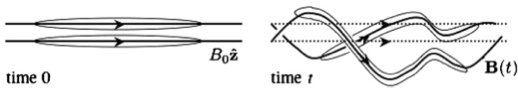
\includegraphics[width=12cm]{figs/slowmodes/slow_parallel_cascade.png}
        \caption{The compressive fluctuations are passively cascaded by the Alfv\'{e}nic
        turbulence, and may remain correlated along the perturbed fieldlines (figure taken
        from Schekochihin et al. \cite{tome}).}
        \label{slowmodes:fig:slow_par}
    \end{center}
    \end{figure}

    In a weakly collisional system like the solar wind, slow modes are subject
    to strong kinetic damping. This is at odds with the observed power law spectra for density and
    field strength fluctuations. Power law spectra suggest that compressive fluctuations undergo a Kolmogorov-style
    turbulent cascade. A possible explanation for this apparent discrepancy is 
    that even though slow modes develop fine scales in the plane perpendicular to the local magnetic
    field as they are passively mixed by the background Alfv\'{e}nic turbulence, they
    remaining correlated in the parallel direction \cite{tome}. 
    This leads to highly
    anisotropic structures with the parallel wavelength set by the initial conditions,
    which results in weak damping since the damping rate is proportional to the parallel
    wavenumber (see \figref{slowmodes:fig:slow_par}). However, this argument ignores 
    dissipation. Lithwick and Goldreich \cite{lithwick01}
    argued against this suggestion, by 
    noticing that when the cascade reaches the ion Larmor radius in the perpendicular
    plane, these highly anisotropic fluctuations would decorrelate due to finite Larmor
    radius effects (which in our model show up as a diffusive term at small perpendicular
    scales), and acquire the same parallel correlation
    lengths as the Alfv\'{e}n waves. Recent observations of the solar wind seem to support the idea that there is no
    parallel cascade \cite{chen11}. However, these results are somewhat inconclusive. In Chen
    \etal\, \cite{chen11}, they construct a representative eddy for the field strength
    fluctuations, and find it to be much more anisotropic than the Alfv\'{e}nic eddy (see
    their figures 4 and 6), which on its surface seems to have settled the issue. But in
    the same paper, they also observe a power law spectrum in the direction of the local
    magnetic field,
    with a spectral exponent between $-1.42$ and $-1.58$ (see their figure 5)---a shallower spectrum than
    that for Alfv\'{e}nic fluctuations (though severely limited by resolution). In fact
    they use this shallow spectrum to construct the eddy in
    the first place. A possible conciliation between these two mutually contradictory
    results is that the compressive fluctuations are
    anisotropic at the outer scale itself, and then cascade to smaller perpendicular and
    parallel scales \cite{chen14}---i.e., an anisotropic structure observed at small
    scales does not imply a lack of parallel cascade, and might be a result of the
    initial conditions.
    This however, still leaves two questions unanswered ---
    \begin{inparaenum}[(a)]
    \item is there a parallel cascade for the compressive fluctuations?
    \item If there is a parallel cascade, why are the compressive fluctuations undamped?
    \end{inparaenum}
    
    We show, using direct numerical simulations of kinetic reduced MHD, that the
    compressive fluctuations undergo a parallel cascade\footnote{The observed parallel
    cascade may be a result of our forcing---this requires further investigation. However,
    the results from \chapref{chap:pp0} explain the observed power law density fluctuation
    spectra for the case where there is no parallel cascade.}, but they remain
    undamped due to suppression of phase mixing by the turbulent plasma echo discussed in
    \chapref{chap:phmixnl}.

\section{Numerics} 

We solve \eqsand{intro:krmhd:els}{intro:krmhd:gpm} using \Gand. Alfv\'{e}n waves were
driven by injecting random velocity fluctuations using a Gaussian white noise source; 
compressive fluctuations were sourced independently by driving $\dBpar$, i.e. the zeroth
velocity moment of $g_B$ (see \eqref{eqs:eq:gnBdef}). The ion charge ($Z$), ion to electron
temperature ratio ($\tau$) and the ion plasma beta ($\beta_i$) were all set to 
one---these choices are representative of the usual solar wind parameters.
The resolution in the real space was
chosen to be $128^3$, $144$ Hermite moments of the perturbed distribution function were
evolved, hypercollisions ($\nu m^8$) and hyperviscosity
($\eta k_\perp^{16}$) were used to regularize fine scale structure.

\section{Alfv\'{e}nic turbulent cascade}

\begin{figure}
\begin{center}
    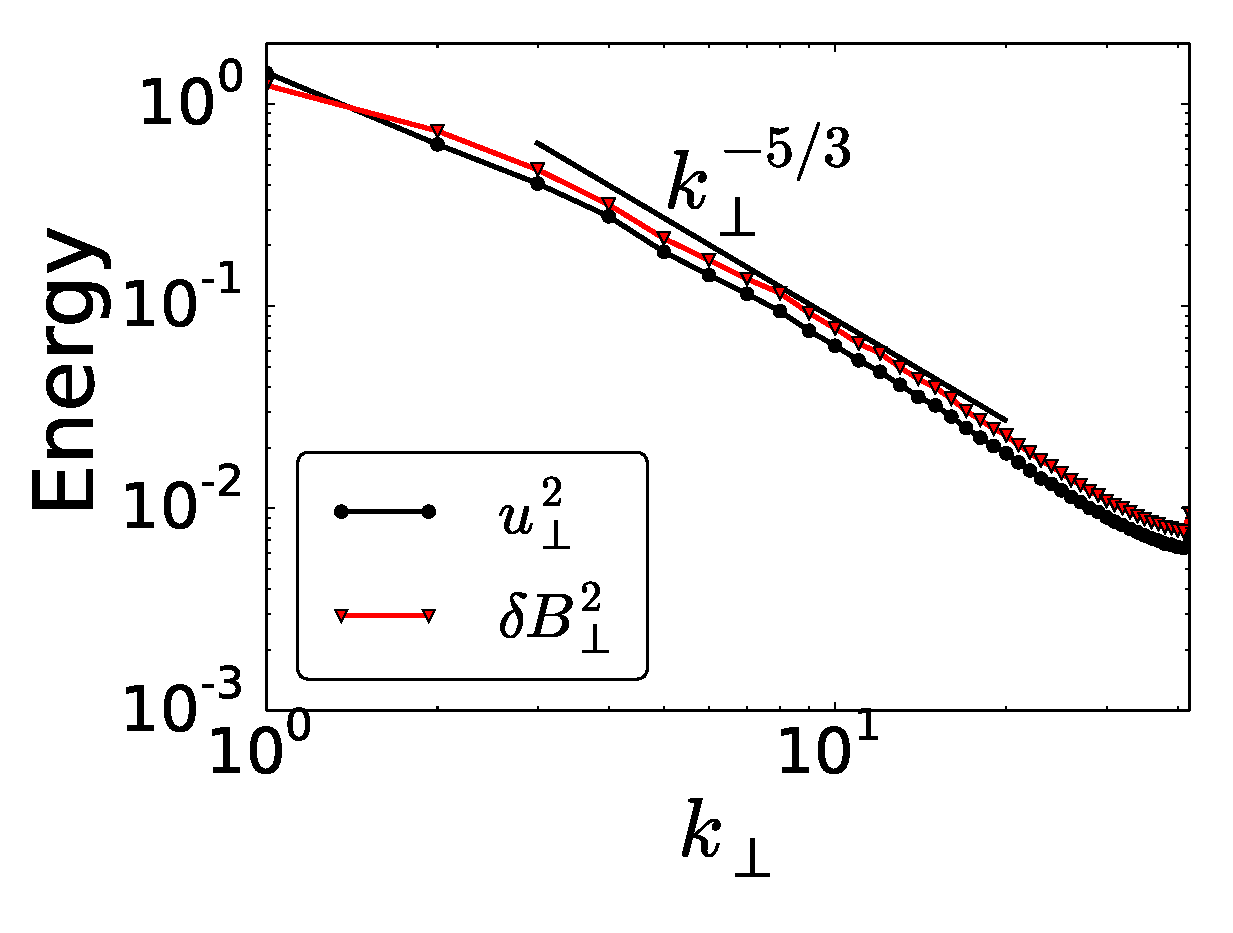
\includegraphics[width=7.4cm]{figs/slowmodes/sw1_alf_kpspec.eps}
    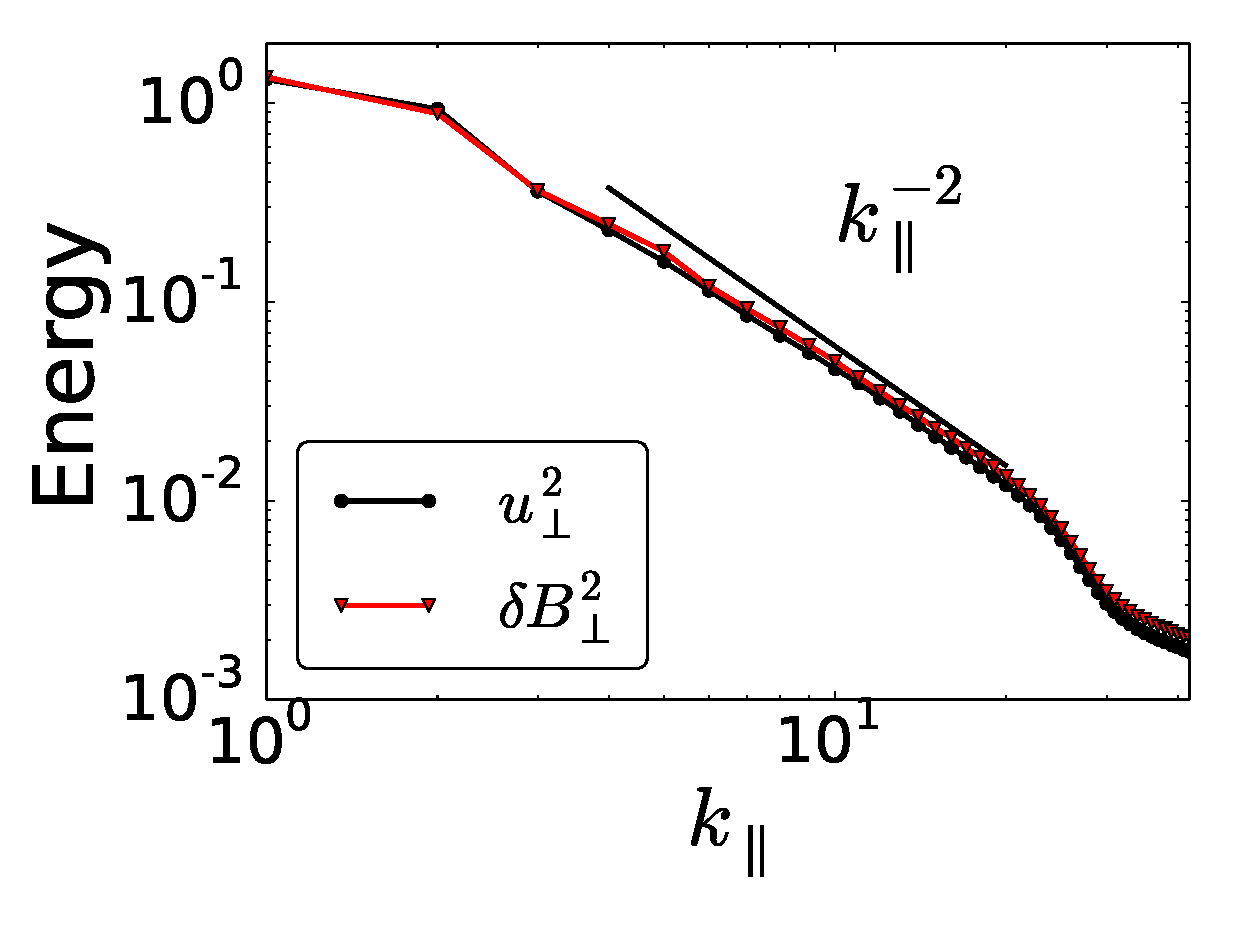
\includegraphics[width=7.4cm]{figs/slowmodes/sw1_alf_kparspec.eps}
    \caption{Perpendicular and parallel spectra of the Alfv\'{e}nic fluctuations. The
    critical balance predictions: $k_\perp^{-5/3}$ for the perpendicular spectra and
    $\kpar^{-2}$ for the parallel spectra are observed in simulations.}
\label{slowmodes:fig:alfspec} 
\end{center}
\end{figure}

    The Goldreich-Sridhar critical balance theory \cite{goldreich95, goldreich97, tome} predicts the Alfv\'{e}nic turbulence to
    have $k_\perp^{-5/3}$ perpendicular, and $\kpar^{-2}$ parallel spectra. The
    precise spectral exponent is a highly debated issue in the community---Boldyrev
    et al.\cite{boldyrev05, boldyrev06, boldyrev09, boldyrev11} argue that 
    scale-dependent dynamic alignment needs to be included in the critical-balance theory
    for MHD turbulence, which ends up predicting a $k_\perp^{-3/2}$ perpendicular
    spectrum, whereas Beresnyak et al. \cite{beresnyak11, beresnyak11prl} observe the
    Goldreich-Sridhar $k_\perp^{-5/3}$ spectrum in their simulations. The resolution requirements to settle this controversy are
    beyond the capability of present day GPUs, and hence this issue is not addressed in
    our work. In our simulations, we observe the perpendicular spectrum to be $k_\perp^{-5/3}$ (see
    \figref{slowmodes:fig:alfspec}), which we consider to be consistent with the
    theories on either side of this debate.
    The parallel spectrum is seen to be $\kpar^{-2}$ (see
    \figref{slowmodes:fig:alfspec}), which is a
    prediction of both the theories. Our numerical spectra
    are broadly consistent with observations in the solar wind \cite{matthaeus82, bale05,
    podesta07, tessein09, podesta10, chen10, chen11}.

\begin{figure}
\begin{center}
    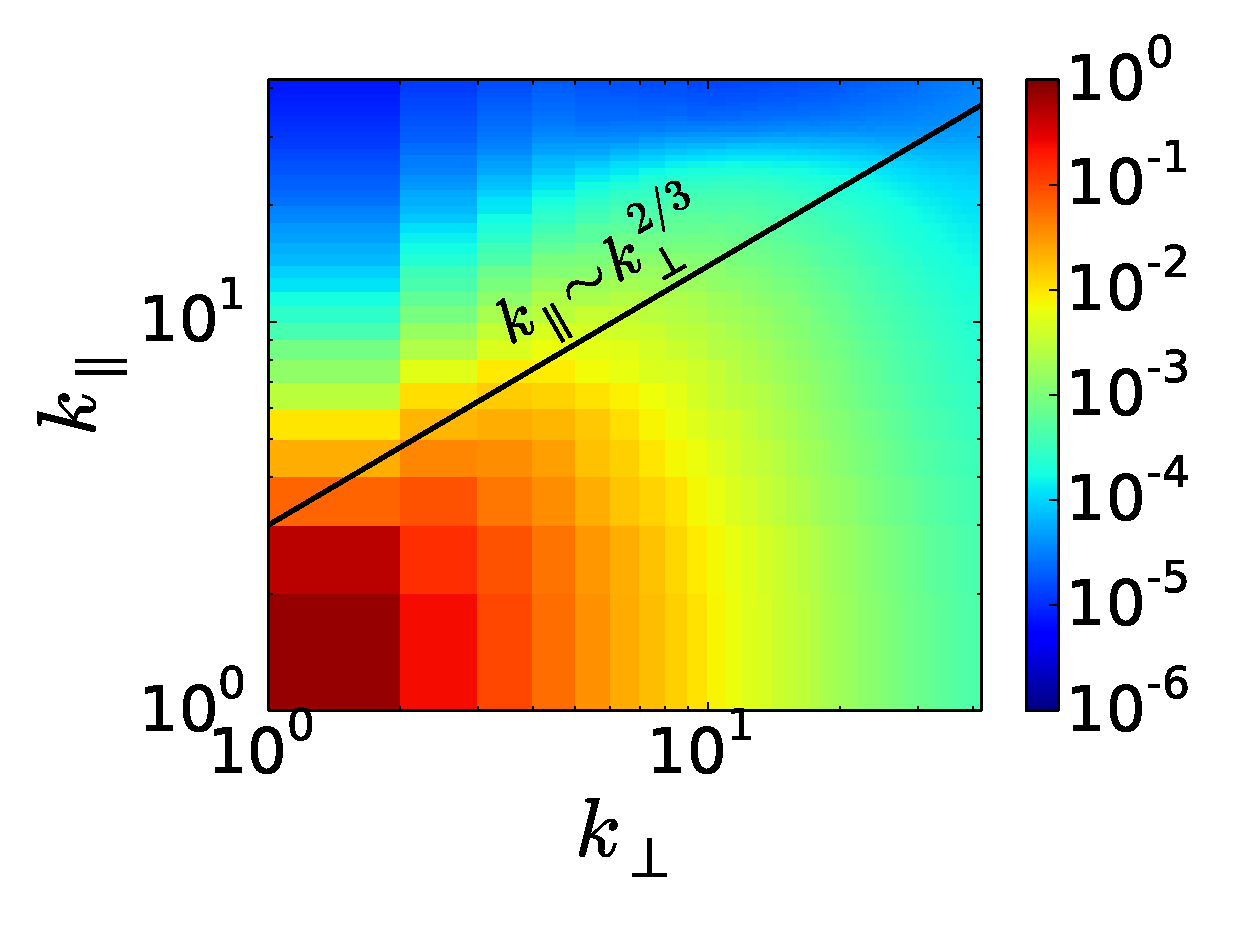
\includegraphics[width=7.4cm]{figs/slowmodes/sw1_u2_kparkp.eps}
    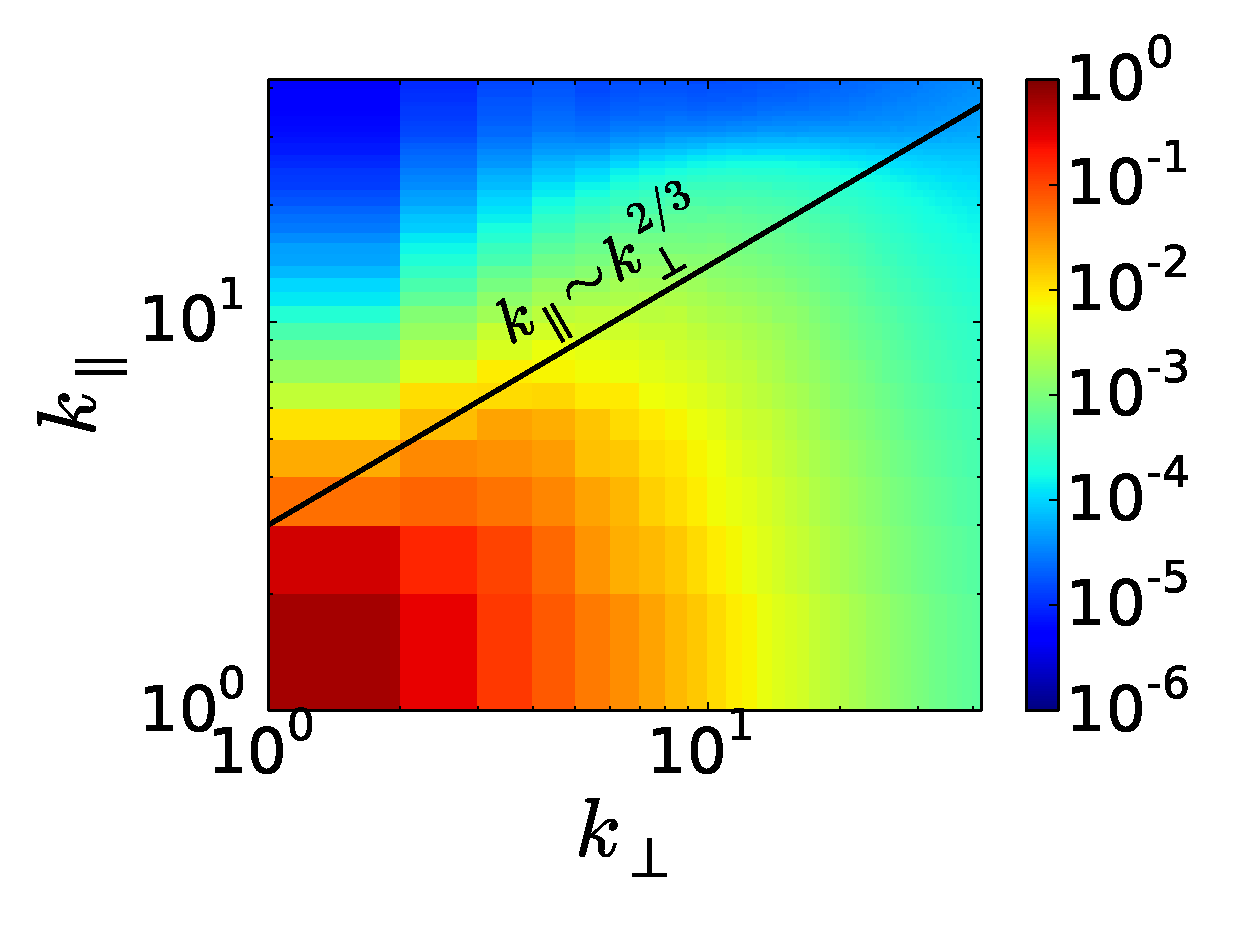
\includegraphics[width=7.4cm]{figs/slowmodes/sw1_b2_kparkp.eps}
    \caption{Kinetic (left) and magnetic (right) energy  vs $k_\perp, \kpar$.}
\label{slowmodes:fig:alfanis} 
\end{center}
\end{figure}

    In addition to the power law spectra having different spectral exponents in the
    perpendicular and the parallel directions, the wavenumber anisotropy predicted by
    critical-balance can also be seen in the 2D spectra plotted in
    \figref{slowmodes:fig:alfanis}. The energy containing region is seen
    to bounded by the $\kpar \sim k_\perp^{2/3}$ line as predicted by critical
    balance\footnote{The anisotropy constant given by the ratio $\kpar/k_\perp^{2/3}$ used
    here is not predicted by critical balance. We use the constant measured in numerical
    simulations by Beresnyak \cite{beresnyak11} to plot the analytical predictions in
    \figref{slowmodes:fig:alfanis}.}.

\section{Slow mode turbulent cascade}

\begin{figure}
\begin{center}
    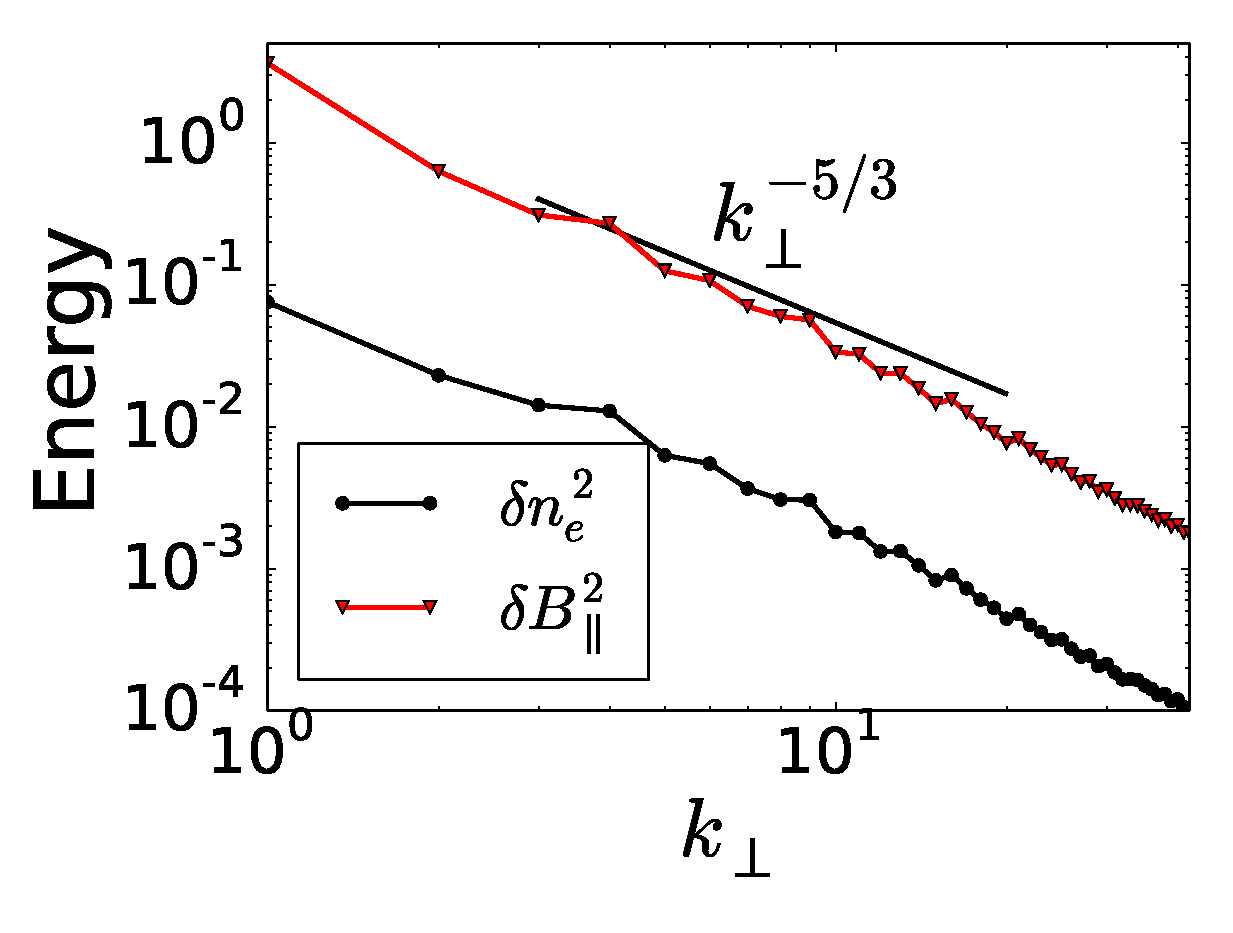
\includegraphics[width=7.4cm]{figs/slowmodes/sw1_dne_kpspec.eps}
    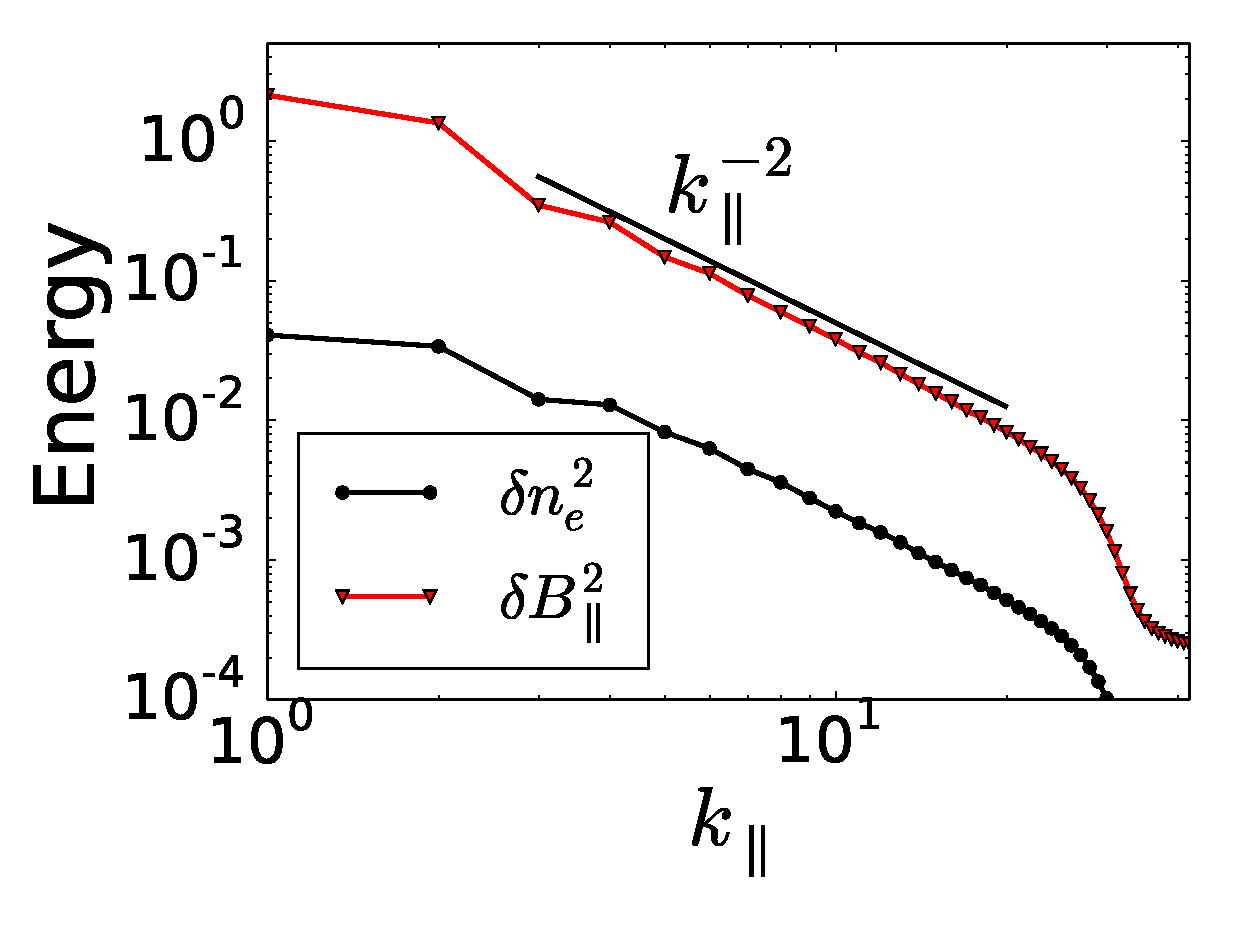
\includegraphics[width=7.4cm]{figs/slowmodes/sw1_dne_kparspec.eps}
    \caption{Perpendicular and parallel spectra of the density and field strength
    fluctuations. The compressive fluctuations being passively mixed, inherit the same perpendicular spectrum as the Alfv\'{e}nic
    fluctuations, consistent with the theoretical prediction. 
    The parallel spectra for compressive modes are also observed to
    be the same as that for the Alfv\'{e}nic perturbations, indicating that the compressive
    fluctuations undergo a parallel cascade, with the parallel correlation lengths being
    set by the Alfv\'{e}nic turbulence.}
\label{slowmodes:fig:dnespec} 
\end{center}
\end{figure}

\begin{figure}
\begin{center}
    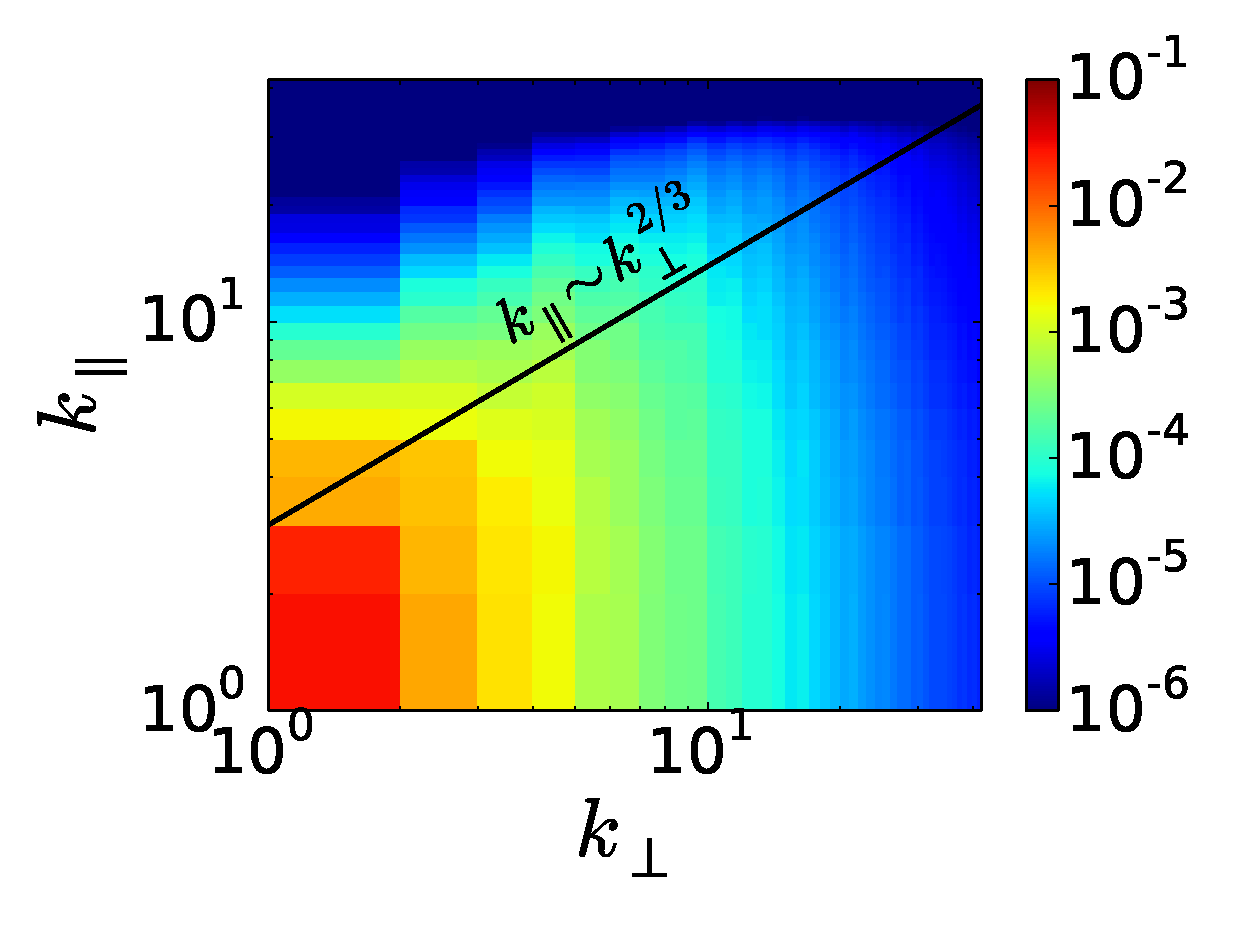
\includegraphics[width=7.4cm]{figs/slowmodes/sw1_dne_kparkp.eps}
    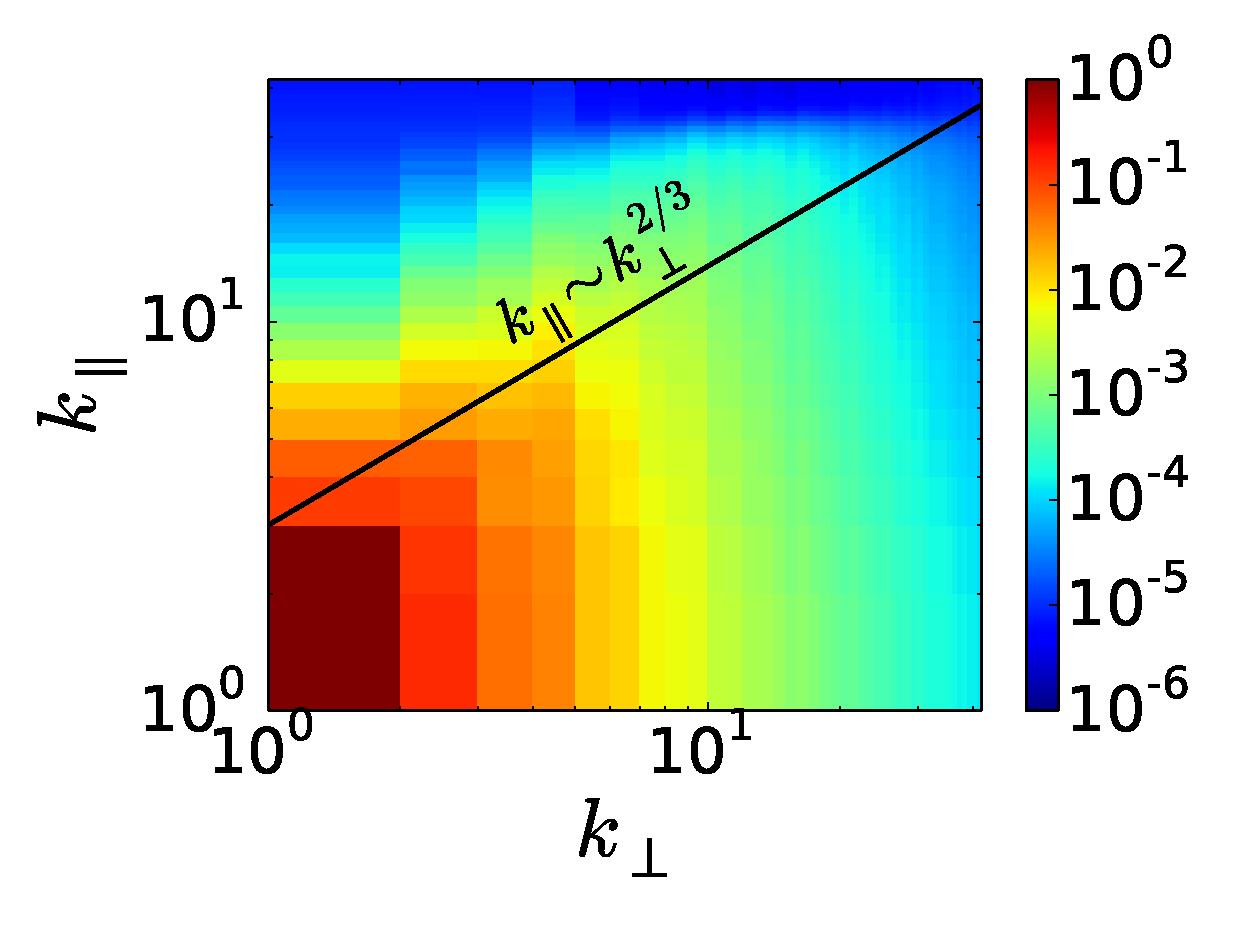
\includegraphics[width=7.4cm]{figs/slowmodes/sw1_dbpar_kparkp.eps}
    \caption{Density (left) and field strength fluctuations (right) vs $k_\perp, \kpar$.}
\label{slowmodes:fig:dneanis} 
\end{center}
\end{figure}

\begin{figure}
\begin{center}
    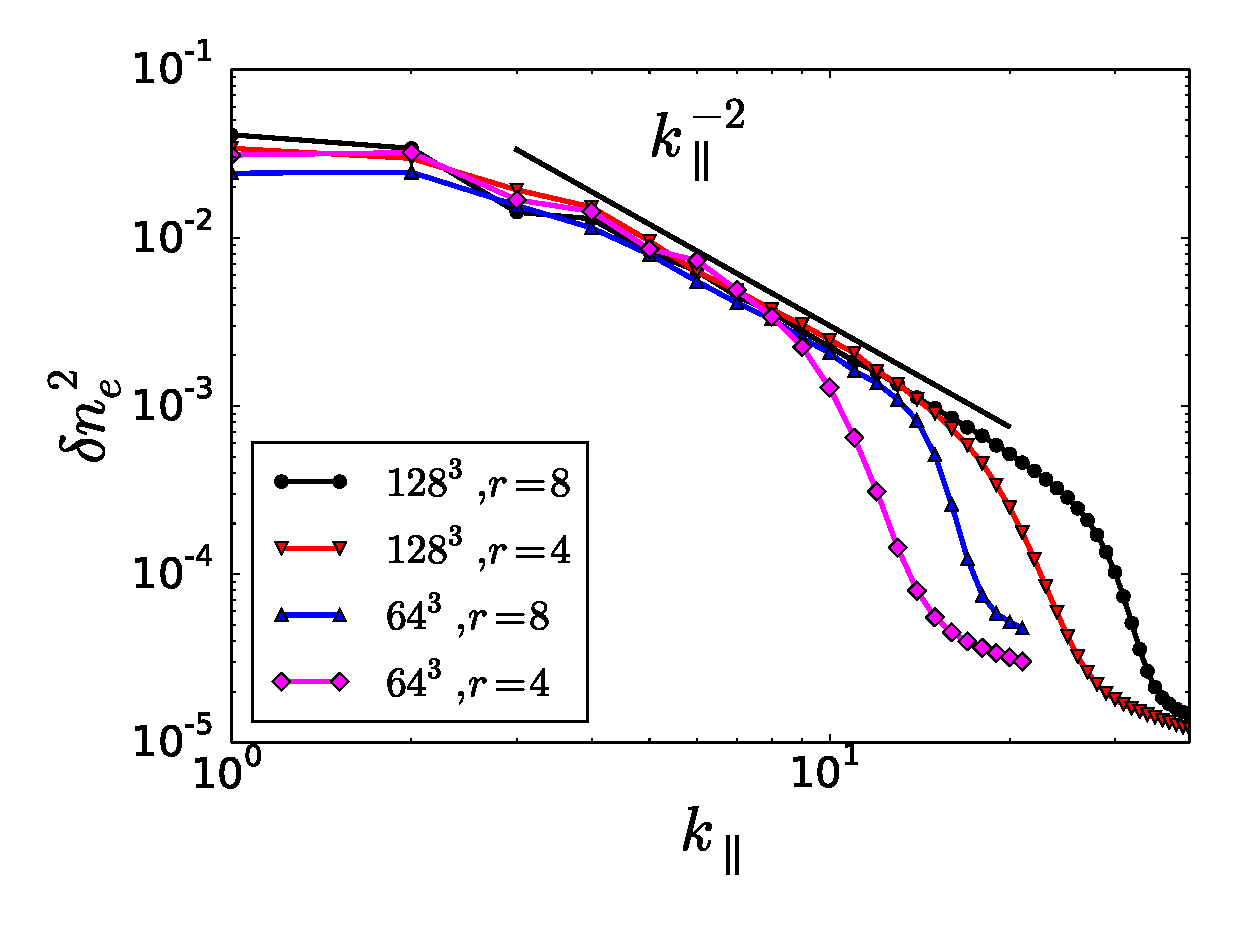
\includegraphics[width=7.4cm]{figs/slowmodes/dneconv_kz.eps}
    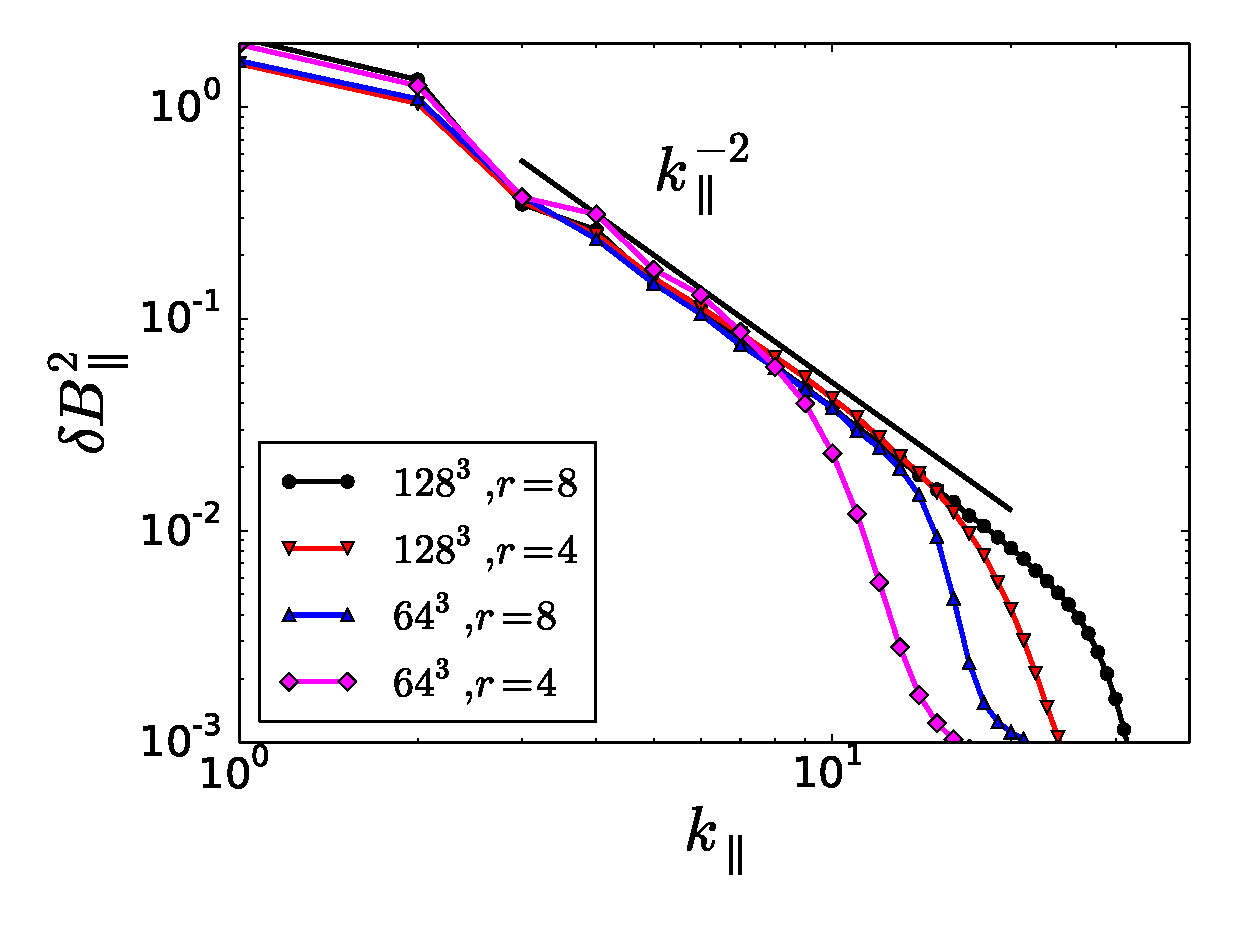
\includegraphics[width=7.4cm]{figs/slowmodes/dbparconv_kz.eps}
    \caption{Density (left) and field strength spectra (right) vs $\kpar$, for different
    resolutions and hyper-dissipation exponents---similar to
    \figref{gandalf:fig:alfconv}. The first number corresponds to the resolution used, the
    second number is the hyper-diffusion exponent.}
    \label{slowmodes:fig:dneconv}
\end{center}
\end{figure}
    
    Being passively mixed, the compressive fluctuations are
    predicted to have the same perpendicular spectrum as the Alfv\'{e}nic fluctuations,
    $k_\perp^{-5/3}$. This is
    observed in our simulations as shown in \figref{slowmodes:fig:dnespec}.
    Interestingly, the compressive fluctuations are also observed to undergo a parallel cascade (see
    \figsand{slowmodes:fig:dnespec}{slowmodes:fig:dneanis}), and have the same parallel spectra as the
    Alfv\'{e}nic cascade. These are preliminary results, and we are still in the process
    of diagnosing the reasons behind such a parallel cascade. However, we carried out a convergence study (see
    \figref{slowmodes:fig:dneconv}), and are fairly confident in our numerical results.
    
    These results show that compressive fluctuations are unable to stay correlated along
    the perturbed fieldlines as suggested by Schekochihin et al. \cite{tome}, and do
    develop small scale structure along the perturbed magnetic field. However, it is not yet clear as to why despite cascading to small parallel scales, the slow modes remain undamped. 

\section{Suppression of phase-mixing}

    We saw in \chapref{chap:phmixnl}, that for a kinetic passive scalar being nonlinearly
    advected by a chaotic velocity field, phase mixing is significantly suppressed due to
    the turbulent plasma echo. In this section we argue that even though compressive 
    fluctuations develop small spatial structure along the fieldline, and should be
    heavily damped by phase mixing, they remain undamped because of the echo.     
    \begin{figure}
    \begin{center}
        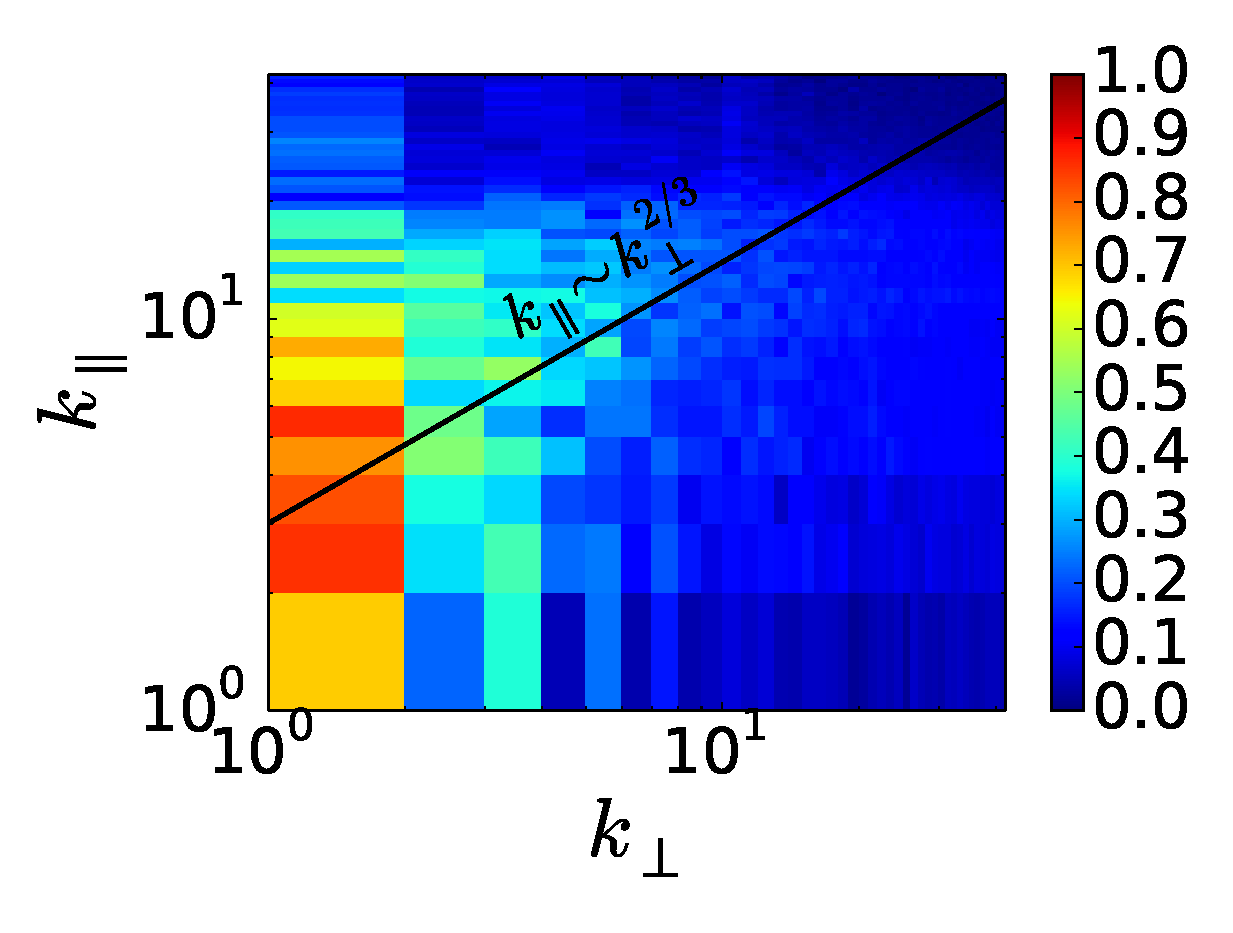
\includegraphics[width=7.4cm]{figs/slowmodes/sw1_gp_m1_supp_vskpkz.eps}
        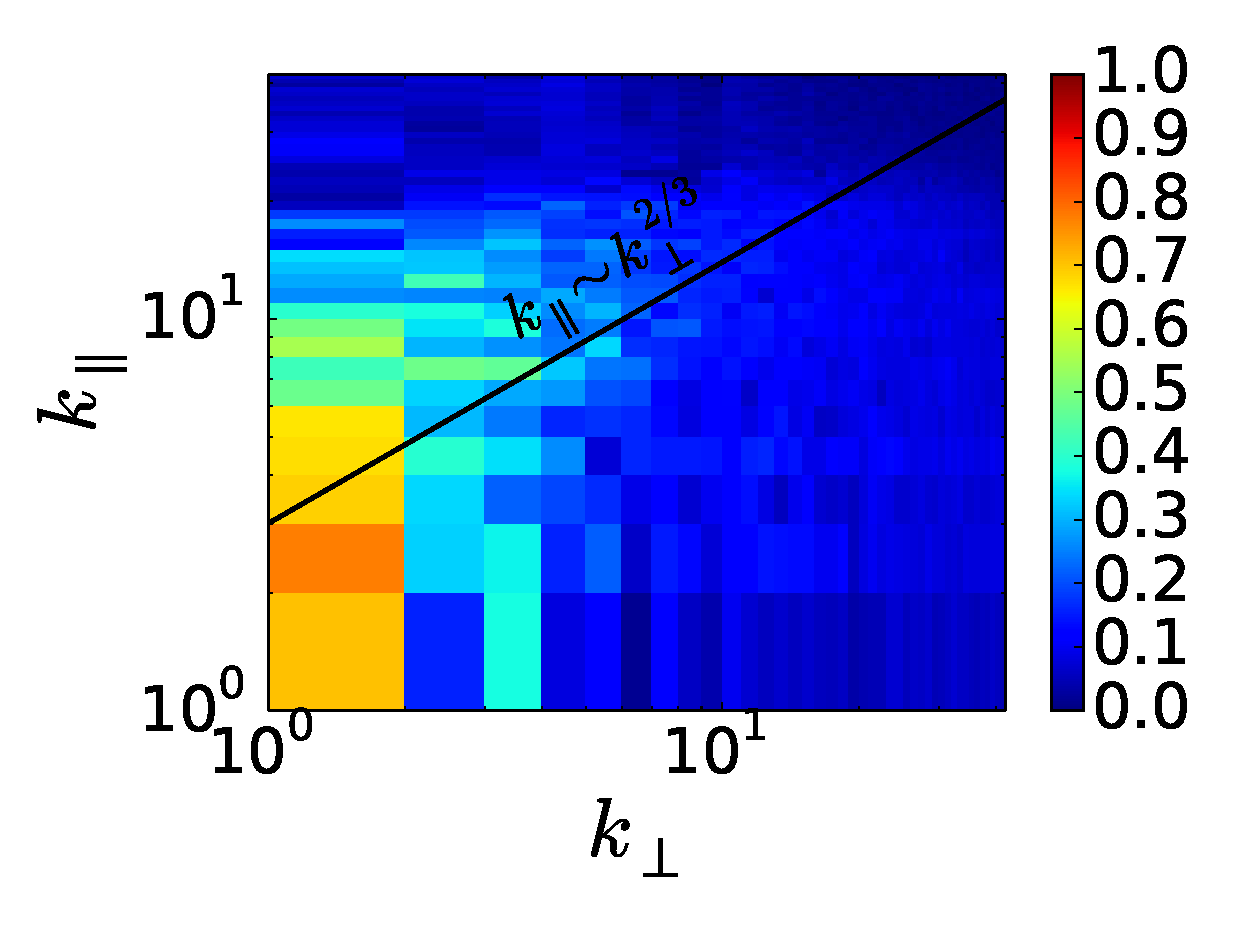
\includegraphics[width=7.4cm]{figs/slowmodes/sw1_gm_m1_supp_vskpkz.eps}
        \caption{Normalized flux  vs
        $k_\perp-\kpar$, at $m=1$  for $g^+$ on the left, and $g^-$ on the right (see
        \eqref{eqs:krmhd:gpmdef}). Phase-mixing is nearly completely suppressed in the
        critical-balance cone, $\kpar \lesssim k_\perp^{2/3}$.}
    \label{slowmodes:fig:supp} 
    \end{center}
    \end{figure}

    We diagnose the plasma echo using the normalized flux diagnostic developed in \chapref{chap:phmixnl}
    (see discussion after \eqref{phmixnl:eq:Fskpm}), except, we use the exact form for the
    flux: $\Gsk~=~\lt|\kpar\rt| \vth \sqrt{(m+1)/2} \, \Re \langle
\tg_{m+1,\mb{k}} \tgmk^\star \rangle$---we do so because the approximate expression for the flux is
valid only at large values of $\sqrt{m}$, and we wish to diagnose the amount of flux out
of the first Hermite moment.
In steady state, the flux to higher Hermite moments is seen to be nearly zero 
(see \figref{slowmodes:fig:supp})---this is especially true in the critical balance cone
$\kpar \lesssim k_\perp^{2/3}$, which is the energy containing region for our system.
    Since, in steady state, the amount of energy transferred to 
    higher Hermite moments out of the first moment is
    nearly zero, the compressive fluctuations have a fluid-like turbulent cascade that
    remains unaffected by phase mixing. As a result, we observe power law spectra for
    density and field strength fluctuations extending all the way to the ion Larmor radius.

\section{Conclusions}
    
    Preliminary results from direct numerical simulations of the kinetic reduced MHD
    equations show
    that compressive fluctuations undergo a parallel cascade in the inertial range, and
    they do not maintain long correlations along the perturbed field as suggested by
    Schekochihin et al \cite{tome}. This also suggests that the anisotropic eddies
    observed in the solar wind \cite{chen11} are probably due to the anisotropy at the
    outer scale---unfortunately, since our analytical, and numerical framework does not
    include the outer scale, this can not be tested in our simulations. 

    Despite the parallel cascade, the compressive fluctuations remain undamped in the
    inertial range, which contradicts the linear prediction that these fluctuations should
    be heavily damped due to transit-time damping. This happens because the Alfv\'{e}nic turbulence drives a
    substantial return flux for the compressive fluctuations from small to large velocity
    space scales (similar to the echo in \chapref{chap:phmixnl})---as a result, phase
    mixing is suppressed, and power law spectra for density and field strength
    fluctuations are observed.
